\chapter{Einleitung}
\ihead[]{Einleitung}
\begin{spacing}{1.1}
	
\noindent Das ist ein Demozitat. (vgl. \cite{link:oculus_headtracking_sensors}) Die Mathematikumgebung kann in \LaTeX\ ebenfalls verwendet werden: $1+1=2$ oder 360$^{\circ}$.
Es können auch Fußnoten gesetzt werden: \texttt{Tabel}\footnote{https://tabel.withgoogle.com} ist ein Projekt von Google. \\ \\
Im Folgenden wird beim Zitat auch der Verweis zur jeweiligen Seite angezeigt: \cite[S. 1]{book:gibson1986ecological} oder \cite[S. 2-4]{corbillon2016viewport}. \\
Nun wird eine neue Seite begonnen. \newpage

\section{Unterkapitel}
\label{sec:unterkapitel1}
Im Folgenden wird eine Abbildung eingebunden:
\begin{figure}[!h]
	\centering
	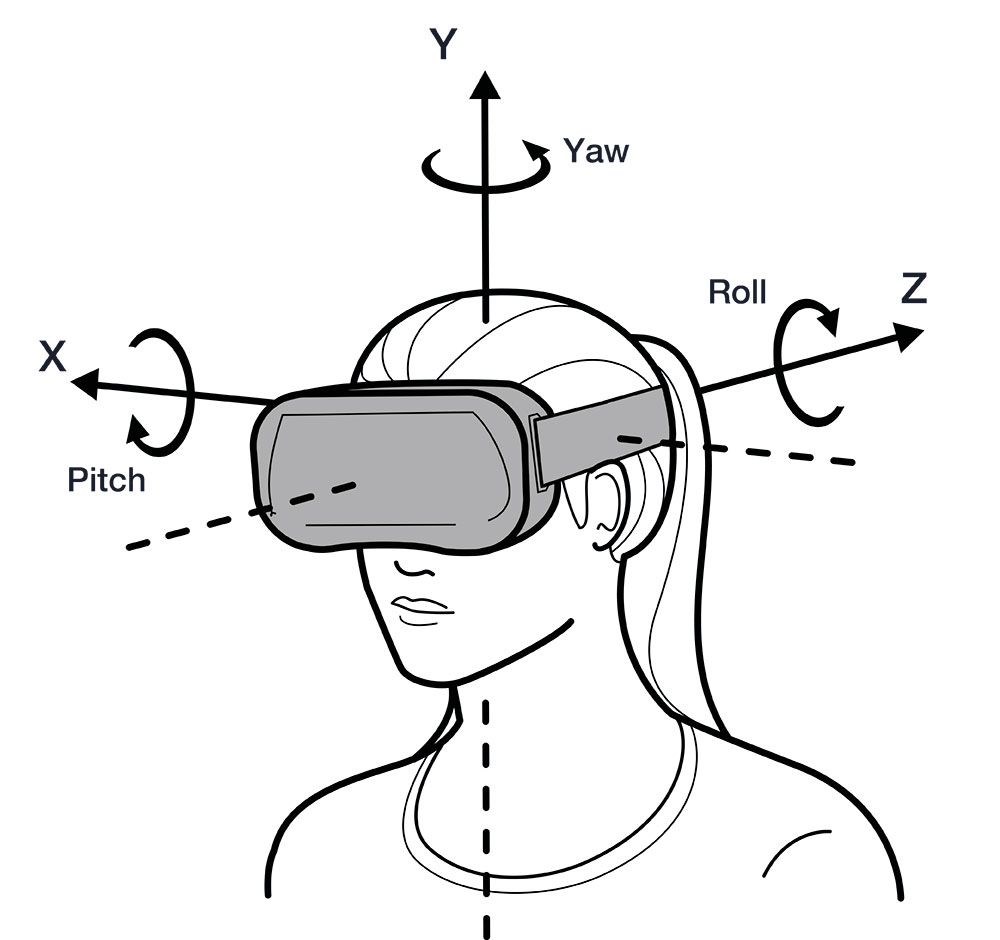
\includegraphics[width=7cm]{images/pyr_coordinates.jpg}
	\caption{Pitch Yaw Roll Koordinaten \cite{link:oculus_headtracking_sensors}}
	\label{picture:pyr_coordinates}
\end{figure}

\noindent Kapitel, Abbildungen etc. können auch mittels Verwendung des jeweiligen Labels referenziert werden. Z.B.: Siehe Kapitel \ref{sec:unterkapitel1}. In Abbildung \ref{picture:pyr_coordinates} sind die verschiedenen Winkelmaße dargestellt, die z.B. Kopfrotationsdaten beschreiben können. \\
Aufzählungen sehen so aus:
\begin{itemize}
	\setlength\itemsep{0.1em}
	\item Aufzählungspunkt 1
	\item Aufzählungspunkt 2
	\item ...
\end{itemize}
Abkürzungen werden zuerst ins Abkürzungsverzeichnis eingetragen und können dann aufgerufen werden: \ac{JPEG}. Bei späterer Erwähnung der Abkürzung \ac{JPEG} wird die definierte Kurzform übernommen.

\subsection{Unterunterkapitel}
Im Folgenden ist Tabelle \ref{table:factors_and_descriptions} dargestellt. Diese können auch direkt mit \LaTeX\ erstellt werden.
\begin{table}[!h]
	\begin{tabular}{|p{2.7cm}|p{10.5cm}|}\hline
		\rowcolor[gray] {.6} \textbf{Faktor} & \textbf{Beschreibung} \\ \hline
		
		\rowcolor[gray] {.8} \multicolumn{2}{|l|}{\textbf{Unterüberschrift 1}} \\ \hline
		Faktor 1 & Beschreibung 1 \\ \hline
		Faktor 2 & Beschreibung 2 \\ \hline
		\rowcolor[gray] {.8} \multicolumn{2}{|l|}{\textbf{Unterüberschrift 2}} \\ \hline
		Faktor 3 & Beschreibung 3 \\ \hline
		Faktor 4 & Beschreibung 4 \\ \hline
	\end{tabular}
	\caption{Faktoren mit Beschreibung}
	\label{table:factors_and_descriptions}
\end{table}

\end{spacing}